\chapter{Méthode de détection d'anomalies}     % numéroté
\label{chap:methodologie}                   % étiquette pour renvois (à compléter!)

Le cœur de notre travail consiste à proposer une méthode de détection d'anomalies où nous utilisons la représentation latente d'un autoencodeur variationnel. Cette représentation servira ensuite comme base pour notre cadre décisionnel nous permettant de détecter des anomalies dans un ensemble de données constitué d'images.

\section{Les objectifs de l'approche} \label{objectifs_metho}

Le premier objectif de notre approche est de faire la détection d'anomalies sur des données complexes, par exemple des images. Nous considérons une image "anormale" comme une image qui contient un contenu global substentiellement différent des autres images. Par exemple, si nous avons un jeu de données d'images de voitures, nous pouvons considérer une image de chien comme une anomalie. 

Le deuxième objectif que nous poursuivons est d'avoir une approche qui discrimine des anomalies en utilisant un seuil qui s'apparente à un niveau de confiance plutôt qu'à une métrique quelconque qui peut être difficile à établir et à interpréter. Sachant ces objectifs, il faut que notre méthodologie soit en mesure de traiter des données complexes et doit nous donner en sortie un score d'anomalie facile à interpréter.

Tout d'abord, il est pertinent de mentionner que le choix d'utiliser des réseaux de neurones, plus particulièrement des autoencodeurs, est étroitement lié au fait de traiter des données complexes. En effet, les réseaux de neurones ont le potentiel d'apprendre des relations complexes et non-linéaires. De plus, l'architecture du réseau peut être adaptée selon la complexité des données en ajoutant des couches de paramètres. Finalement, les réseaux à convolutions sont également bien adaptés au domaine de la vision numérique en prenant en compte l'information de manière locale dans une image.

Ensuite, l'avantage d'avoir un score d'anomalie facile à interpréter en sortie est de simplifier la prise de décision pour discriminer les anomalies des observations "normales". Pour illustrer cet avantage, prenons un contre-exemple où l'on veut faire la détection d'anomalies à partir d'une méthode basée sur une distance comme les $k$ plus proches voisins. Dans cette approche, nous pourrions considérer comme "anormales" les observations pour lesquelles il y a moins de $k$ voisins à l'intérieur d'un rayon de longueur $\epsilon$. La détection d'anomalie requiert donc de définir les paramètres $k$ et $\epsilon$, qui ne pourront pas être choisis aussi facilement qu'un niveau de confiance. Un score d'anomalie que l'on pourrait interpréter de manière similaire à un niveau de confiance serait effectivement beaucoup plus simple et objectif à déterminer.

\section{Les hypothèses de l'approche}

Dans notre approche, nous supposons que  nous avons accès à un jeu de données d'entraînement $\mathcal{X} = \{\boldsymbol{X^{(1)}}, ..., \boldsymbol{X^{(n)}}\}$ qui contient $n$ observations indépendantes de $\mathbf{X} \in \mathbb{R}^{d_1 \times d_2}$. Afin de simplifier la notation, on suppose que les matrices sont carrées, soit $d_1=d_2=d$. De cette manière, ces matrices peuvent être exprimées comme des vecteurs de longueur $d^2$. On pourrait aisément traiter des matrices où $d_1$ serait différent de $d_2$. Dans notre cas, on peut donc réécrire sous la forme vectorielle $\boldsymbol{x^{(i)}} = [x^{(i)}_1,...,x^{(i)}_{d^2}]$; la façon d'obtenir cette forme vectorielle a peu d'importance, tant qu'on procède toujours de la même manière pour toutes les observations. Ces représentations peuvent être obtenues par ligne ou par colonne. Dans notre cas, nous avons dû procéder à ce genre de transformation pour l'une des approches comparatives testées dans nos applications, soit l'analyse en composantes principales. Pour ce faire, nous avons aplati les matrices (images) en vecteurs. La figure \ref{fig:one_hot} illustre de quelle façon nous pourrions procéder pour des images à un seul canal et des images à trois canaux, ou de type \textit{RGB}.

\begin{figure}[h]
	\centering
	\begin{subfigure}{12cm}
		\centering
		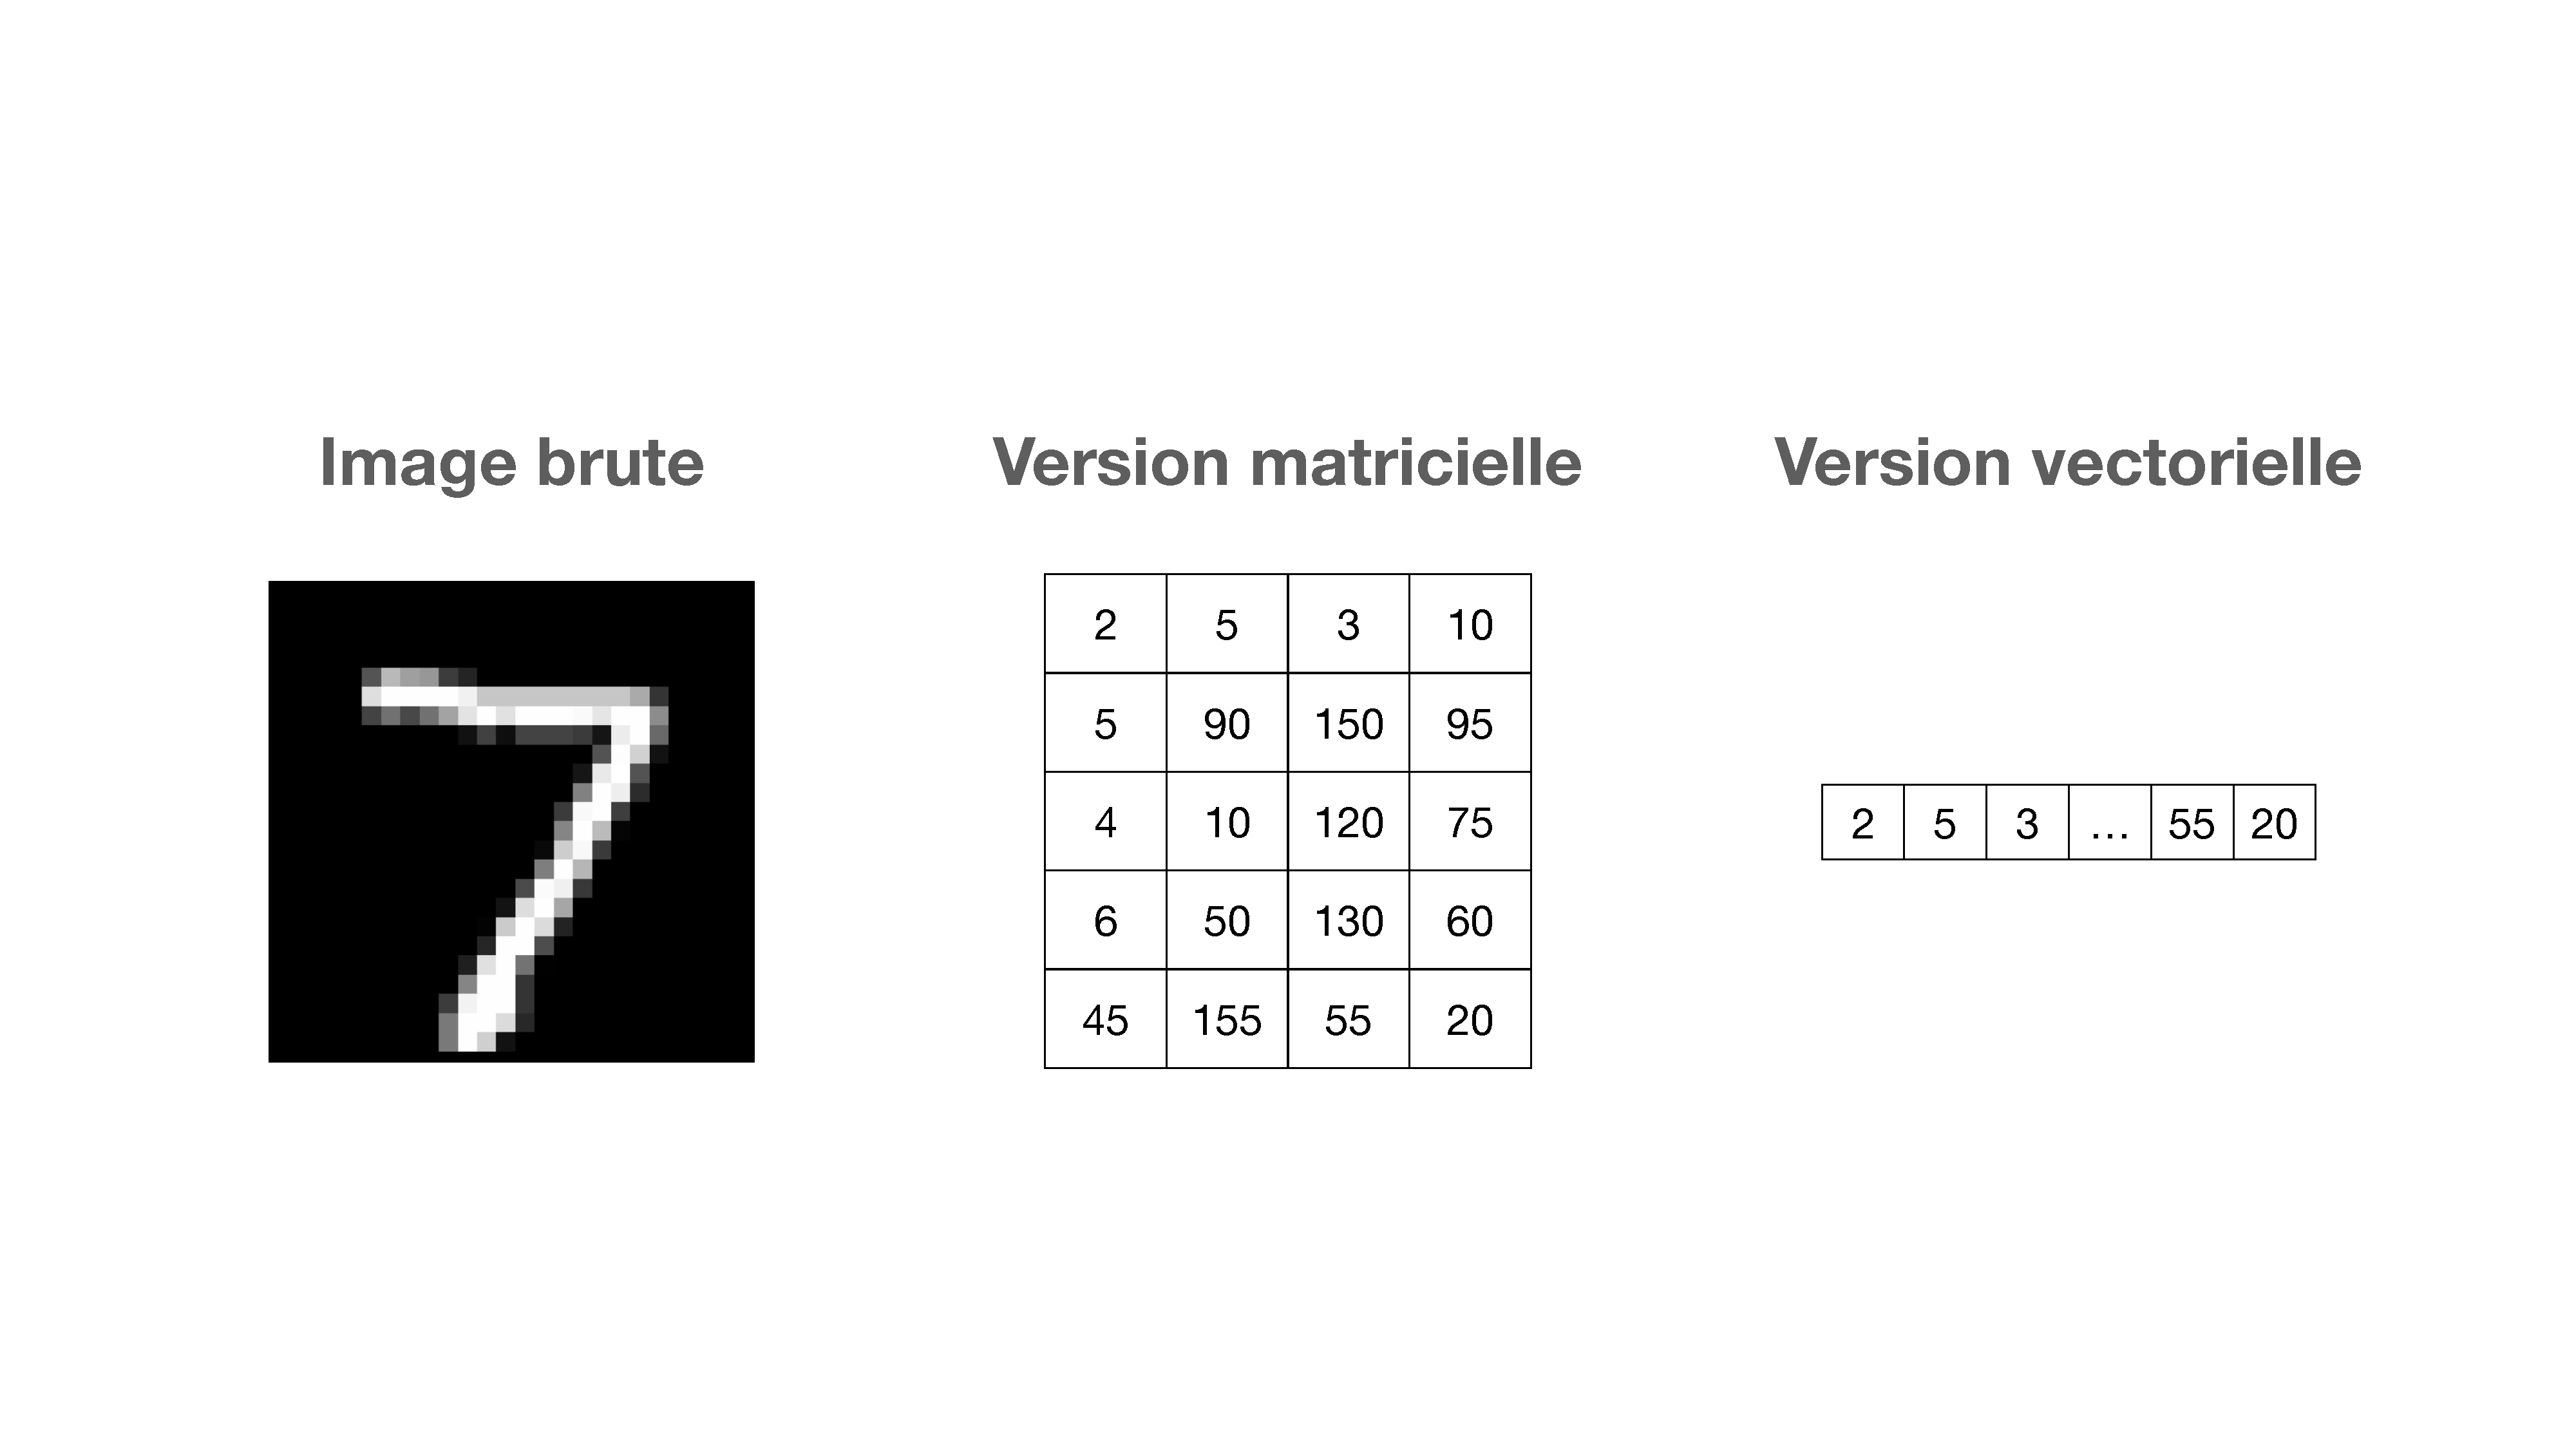
\includegraphics[width=1\linewidth]{images/keynote/one-hot-transfo}
		\caption{Images à un seul canal ("noir et blanc")}
	\end{subfigure}
	\begin{subfigure}{12cm}
		\centering
		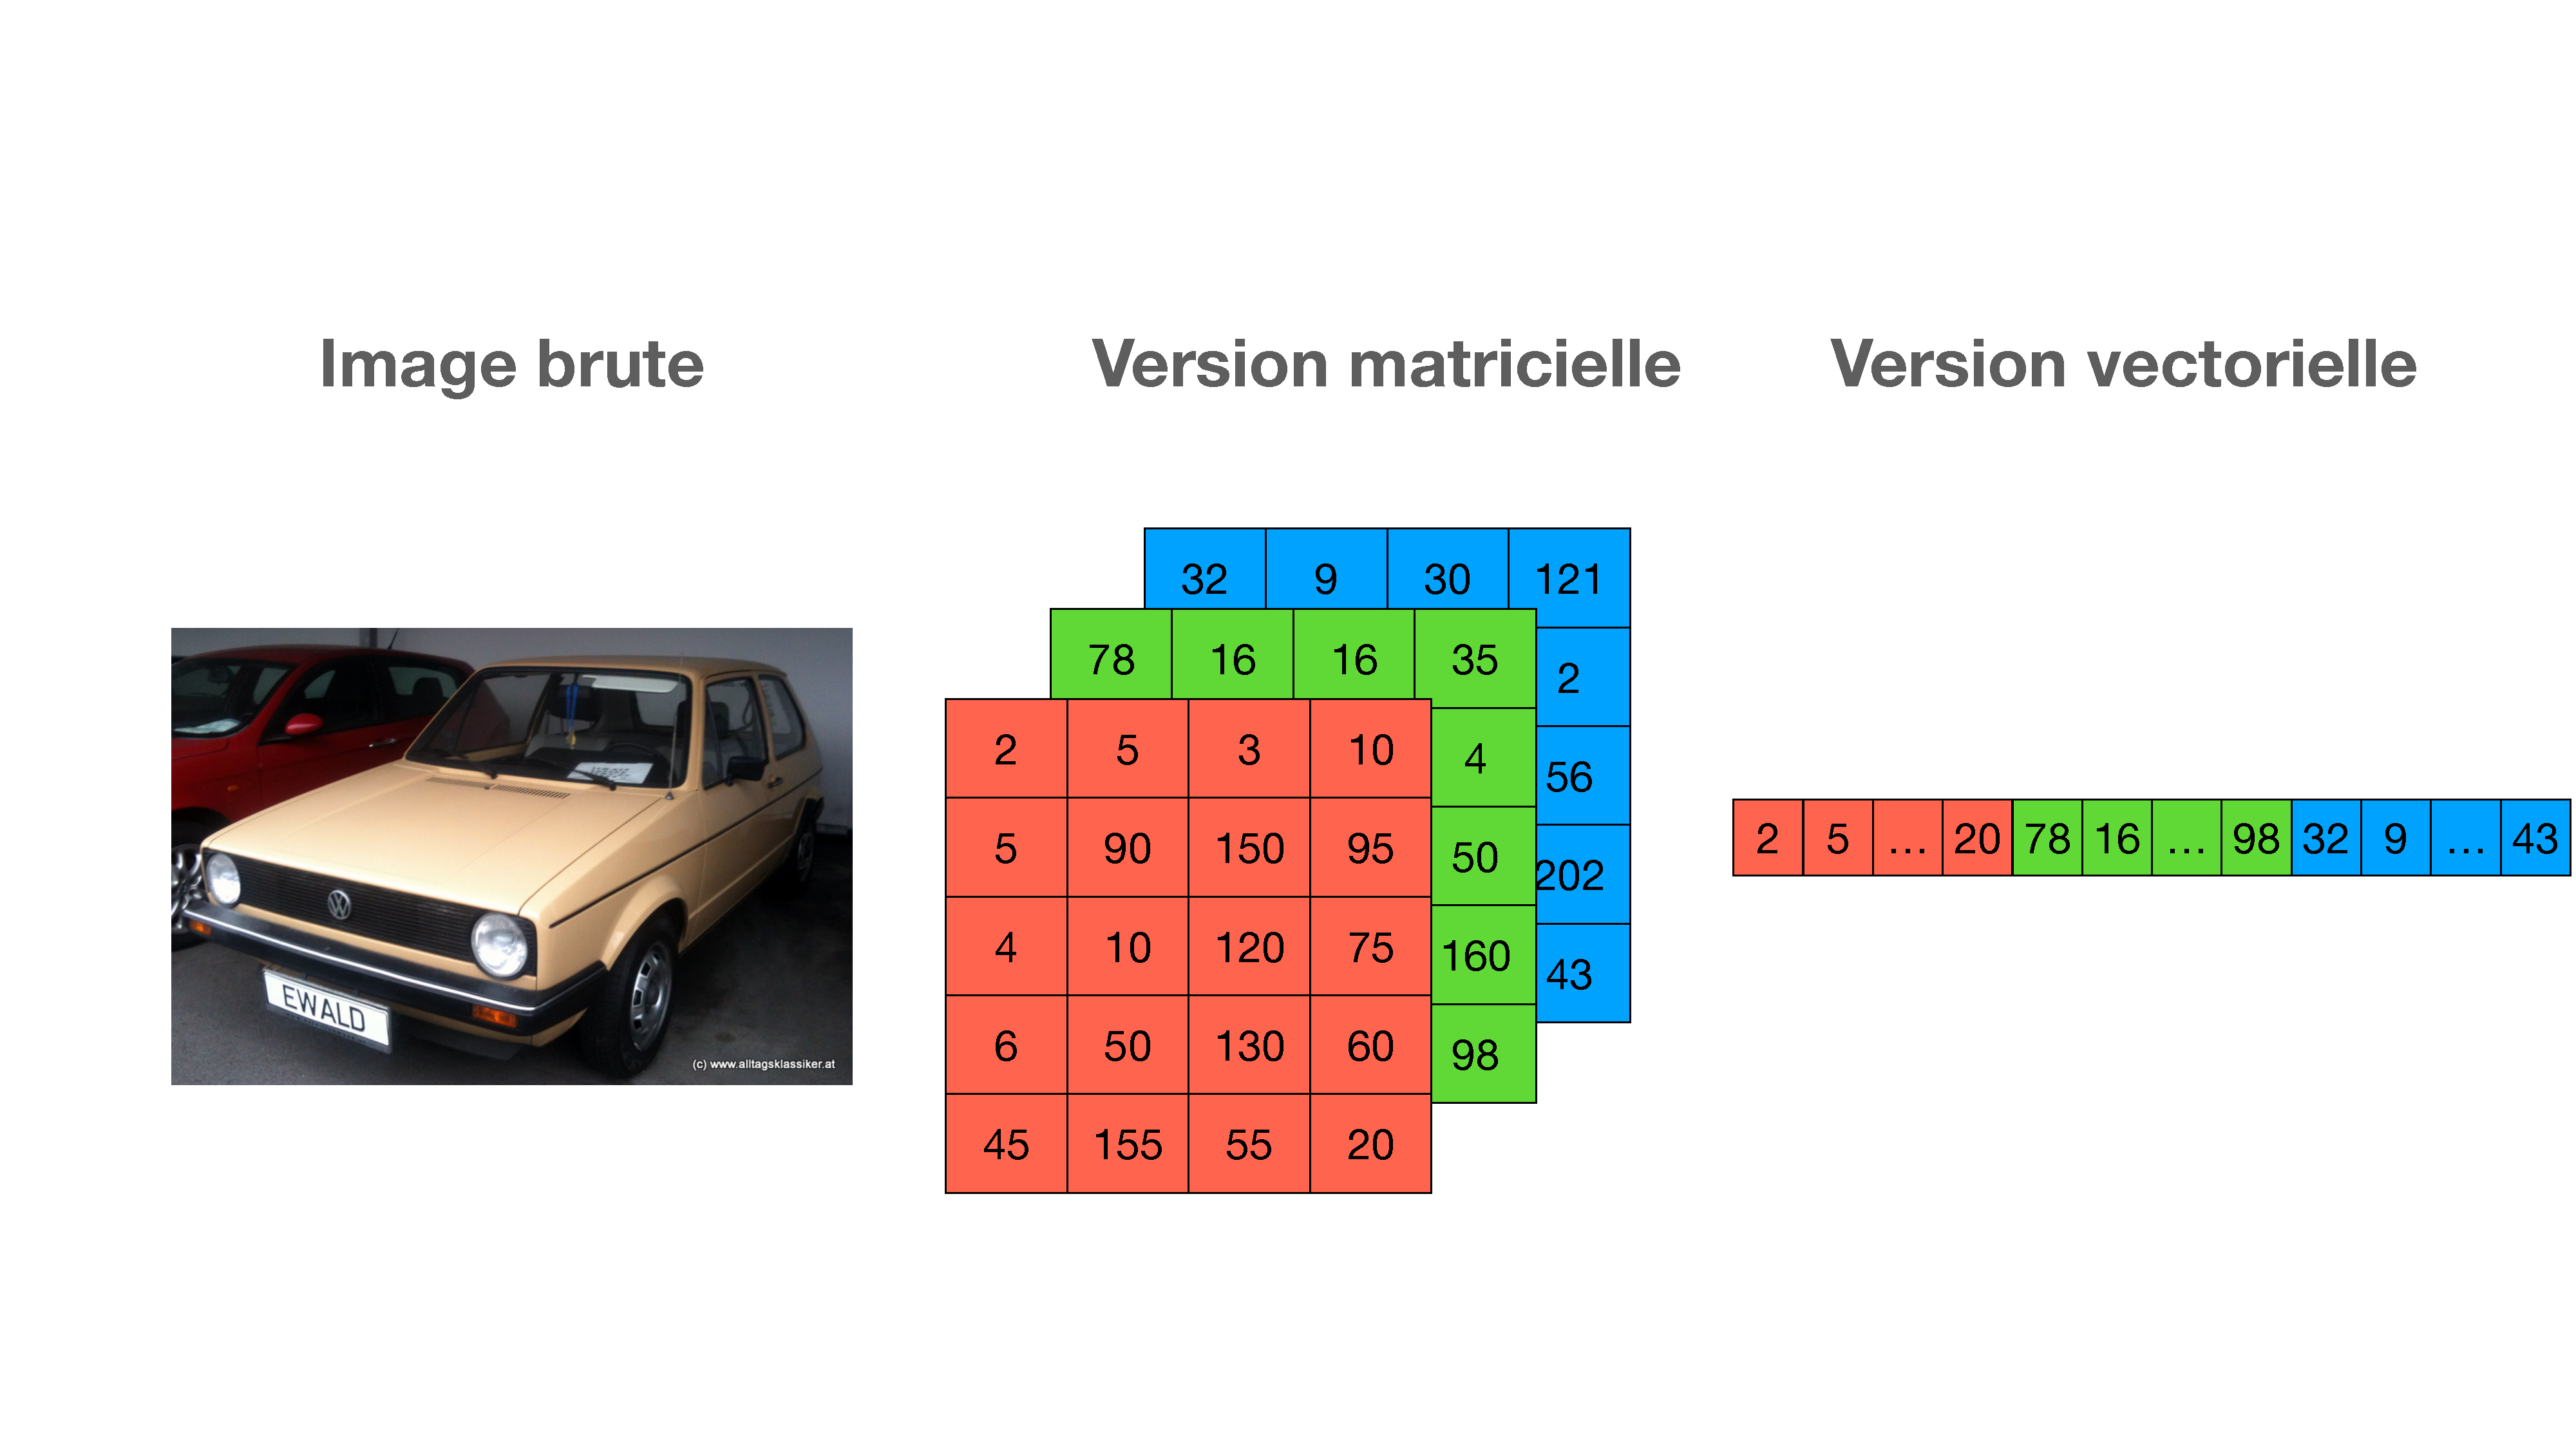
\includegraphics[width=1\linewidth]{images/keynote/one-hot-transfo-rgb}
		\caption{Images à 3 canaux (\textit{RGB})}
	\end{subfigure}
	\caption[Exemple de vectorisation d'une image.]{Figure illustrant une méthodologie pour transformer une image d'entrée brute en format vectoriel selon le nombre de canaux de l'image. Les valeurs présentées dans les matrices sont fictives.}
		\label{fig:one_hot}
\end{figure}


Les $n$ observations de notre jeu d'entraînement proviennent d'un mélange à proportion $(1-p)$ d'observations identiquement distribuées dites "normales" et $p$ d'observations identiquement distribuées dites "anormales". Dans un cas théorique, on pourrait dire que nos observations "normales" proviennent d'un sous-ensemble, disons $\mathcal{N}$, faisant partie de l'ensemble $\mathcal{T}$.  Les observations "anormales", $\mathcal{A}$, peuvent quant à elles provenir du reste de l'ensemble $\mathcal{T}$, soit $\overline{\mathcal{N}} \cap \mathcal{T}$. Cet exemple est illustré à la figure  \ref{fig:exemple_populationsa}. Cependant, dans la pratique il est difficile d'obtenir des images "anormales" couvrant la totalié de l'ensemble $\overline{\mathcal{N}} \cap \mathcal{T}$. Pour nous permettre d'avoir une population d'observations "anormales", nous allons plutôt assumer que nos anomalies proviennent d'un sous-ensemble $\mathcal{A}$, ce qui est illustré à la figure \ref{fig:exemple_populationsb}. 

\begin{figure}[h]
	\centering
	\begin{subfigure}{.33\textwidth}
		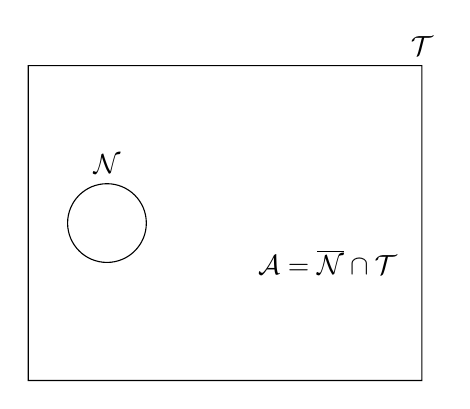
\begin{tikzpicture}[fill=gray]
			\draw (-1,0) circle (0.5) (-1,0.5)  node [text=black,above] {$\mathcal{N}$}
			(1.8,-0.5) node {$\mathcal{A}=\overline{\mathcal{N}} \cap \mathcal{T}$}
			(-2,-2) rectangle (3,2) node [text=black,above] {$\mathcal{T}$};
		\end{tikzpicture}
	\caption{Exemple théorique}
	\label{fig:exemple_populationsa}
	\end{subfigure}
	\hspace{1cm}
	\begin{subfigure}{.33\textwidth}
		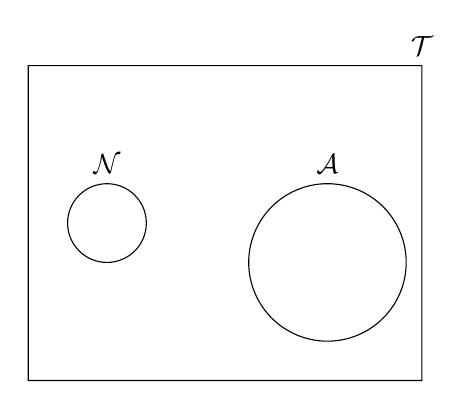
\begin{tikzpicture}[fill=gray]
			\draw (-1,0) circle (0.5) (-1,0.5)  node [text=black,above] {$\mathcal{N}$}
			(1.8,-0.5) circle (1) (1.8,0.5)  node [text=black,above] {$\mathcal{A}$}
			(-2,-2) rectangle (3,2) node [text=black,above] {$\mathcal{T}$};
		\end{tikzpicture}
	\caption{Exemple pratique}
	\label{fig:exemple_populationsb}
	\end{subfigure}
	\caption{Exemple illustrant comment nos ensembles de populations "normales" et "anormales" sont créés dans nos jeux de données.}
	\label{fig:exemple_populations}
\end{figure}

 Pour indiquer si la matrice $\boldsymbol{X^{(i)}}$ provient de la population dite "normale" $\mathcal{N}$, soit $ \boldsymbol{X^{(i)}}\in\mathcal{N}$, on utilise la fonction indicatrice définie ci-dessous,

\begin{gather*}  \label{eq:ind_anomaly}
\delta_{i}=
\begin{cases}
0 & \text{si $\boldsymbol{X^{(i)}}\in\mathcal{N}$} \\
1 & \text{si $\boldsymbol{X^{(i)}}\not\in\mathcal{N}$}.
\end{cases}
\end{gather*}

On suppose que la proportion $p$ est faible, typiquement moins de 5\%. Dans la pratique, nous ne connaissons pas la valeur des $\delta_i$, ce qui veut dire que nous ne pouvons connaître la proportion réelle d'anomalies $p$. 

Nous avons également $k$ observations indépendantes de matrices constituées des mêmes $d \times d$ dimensions dans un jeu de données test $\mathcal{X^*} = \{\boldsymbol{X^{*(1)}},...,\boldsymbol{X^{*(k)}}\}$. On suppose que la proportion d'anomalies $p^*$ dans ce jeu de données est similaire ou différente de $p$. C'est donc dire que parmi ces $k$ observations, $(1-p^*) \times k$ proviennent de la même distribution $\mathcal{N}$ que les données du jeu d'entrainement et une proportion $p^*$ sont des anomalies (également de la même population $\mathcal{A}$ d'anomalies que le jeu d'entrainement). De la même manière que pour le jeu de données d'entraînement $\mathcal{X}$, nous ne savons pas si une matrice $\boldsymbol{X^{*}}$ du jeu de données test provient de la population dite "normale" $\mathcal{N}$. Nous ne connaissons donc pas non plus la proportion réelle $p^*$. Pour indiquer si la matrice $\boldsymbol{X^{*(i)}}$ provient de la population dite "normale" $\mathcal{N}$, soit $ \boldsymbol{X^{*(i)}}\in\mathcal{N}$, on utilise la même fonction indicatrice que celle définie dans l'équation \ref{eq:ind_anomaly}:

\begin{gather}  \label{eq:ind_anomaly}
\delta^{*}_{i}=
\begin{cases}
0 & \text{si $\boldsymbol{X^{*(i)}}\in\mathcal{N}$} \\
1 & \text{si $\boldsymbol{X^{*(i)}}\not\in\mathcal{N}$}.
\end{cases}
\end{gather}


\section{Description de l'approche} \label{section:description}

Notre approche se divise essentiellement en deux étapes. La première étape implique d'entraîner un autoencodeur variationnel pour apprendre les "caractéristiques" de la population normale du jeu de données d'entraînement $\mathcal{X}$. La deuxième étape consiste à définir un cadre décisionnel à partir des représentations latentes de l'autoencodeur entraîné nous permettant ainsi d'identifier les anomalies dans le jeu de données de test $\mathcal{X^*}$ avec seuil $\alpha$ similaire à un niveau de confiance, mais que nous appellerons plutôt \textbf{niveau de filtration}.

\subsection{Entraîner l'autoencodeur} \label{meth:train-vae}

La première étape consiste à utiliser le jeu de données d'entraînement $\mathcal{X}$ pour entraîner l'autoencodeur variationnel. Étant donné que $\mathcal{X}$ ne contient presque pas d'anomalies, cela devrait permettre d'appendre les caractéristiques, ou la distribution, de la population dite "normale". Cette distribution apprise sera contenue dans la représentation latente du VAE entraîné, ou plus spécifiquement dans les couches $\boldsymbol{\mu}$ et $\boldsymbol{\sigma}$ du réseau. Ces deux couches précèdent la couche latente et permettent de générer celle-ci de manière stochastique, comme nous l'avons vu dans la section \ref{background-vae}. Les VAE sont généralement entraînés avec une fonction de coût à deux composantes (voir l'équation \ref{eq:loss_vae}). Une de ces deux composantes est associée à la représentation latente du réseau, s'assurant ainsi que celle-ci s'approche d'une distribution \textit{a priori}, soit une $N(0, I)$ dans notre cas. Pour ce faire, les valeurs des couches $\boldsymbol{\mu}$ et $\boldsymbol{\sigma}$ doivent s'approcher des paramètres de la loi \textit{a priori}, soit les vecteurs $(\mathbf{0}, \mathbf{1})$ = $(\boldsymbol{0_m}, \boldsymbol{1_m})$ dans le cas d'une représentation latente à $m$ dimensions; nous pourrons d'ailleurs tirer avantage de cette hypothèse \textit{a priori} dans notre règle de décision que nous allons décrire en détails à la prochaine section. La deuxième composante de la fonction de perte, soit l'erreur de reconstruction, demeure primordiale dans l'entraînement du réseau. Dans sa forme la plus simple, cette erreur de reconstruction est définie pixel par pixel. Dans le cas de l'erreur quadratique moyenne, cette composante de perte peut être définie pour la contribution d'une observation $i$ comme

\begin{gather} \label{eq:mse_loss}
L(\boldsymbol{x^{(i)}}, p_\phi\{q_\theta(\boldsymbol{x^{(i)}})\}) = \frac{1}{d^2} \sum_{l=1}^{d^2} (x^{(i)}_{l} - p_\phi\{q_\theta(\boldsymbol{x^{(i)}})\}_l)^2,
\end{gather}

où $p_\phi\{q_\theta(\boldsymbol{x^{(i)}})\}_l$ est le $l$-ème élément du vecteur ou de la matrice de sortie $p_\phi\{q_\theta(\boldsymbol{x^{(i)}})\}$ donnée par l'équation \ref{eq:output}. Dans le cas d'une image, le $l$-ème élément correspond au $l$-ème  pixel de l'image.

La fonction de perte définie à l'équation \ref{eq:mse_loss} accorde autant d'importance à chacun des pixels de l'image. C'est donc dire que le réseau a pour objectif de bien reconstruire autant les pixels en arrière-plan que les pixels centraux. Dans notre cas,  on cherche à trouver des anomalies dans le contenu global de l'image. Pour illustrer ce qu'on veut dire par "contenu global", la figure \ref{fig:exemple_global} montre quelques exemples d'images considérées comme "normales" et "anormales". Dans la figure \ref{fig:exemple_global}, on peut y voir que les images "normales" de la sous-figure \ref{fig:sfig1} correspondent à des voitures dans un environnement extérieur. La sous-figure \ref{fig:sfig2} présente des images "anormales", où l'on peut apercevoir des chiens dans un environnement extérieur. Même si l'arrière-plan de ces images est similaire à celui de \ref{fig:sfig1}, le contenu global correspond à des images de chiens et non de voiture. À l'opposé, on peut apercevoir à la sous-figure \ref{fig:sfig3} des images de voitures correspondant à des modèles particuliers, des environnements intérieurs et aussi contenant des écritures sur les marges supérieures et inférieures de l'image. Malgré ces observations, le contenu global de ces images correspond tout de même à des voitures, ce qui nous amène à les considérer comme des images dites "normales".

\begin{figure} [htb]
	\begin{subfigure}{.33\textwidth}
		\centering
		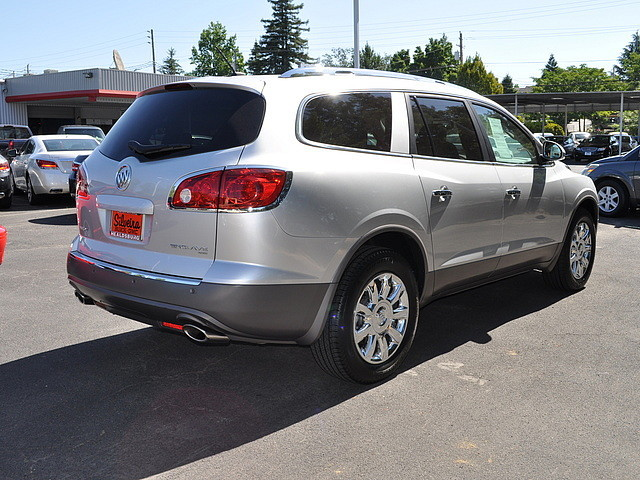
\includegraphics[width=.8\linewidth,height=3cm]{images/images_anomalies/inlier-1}
		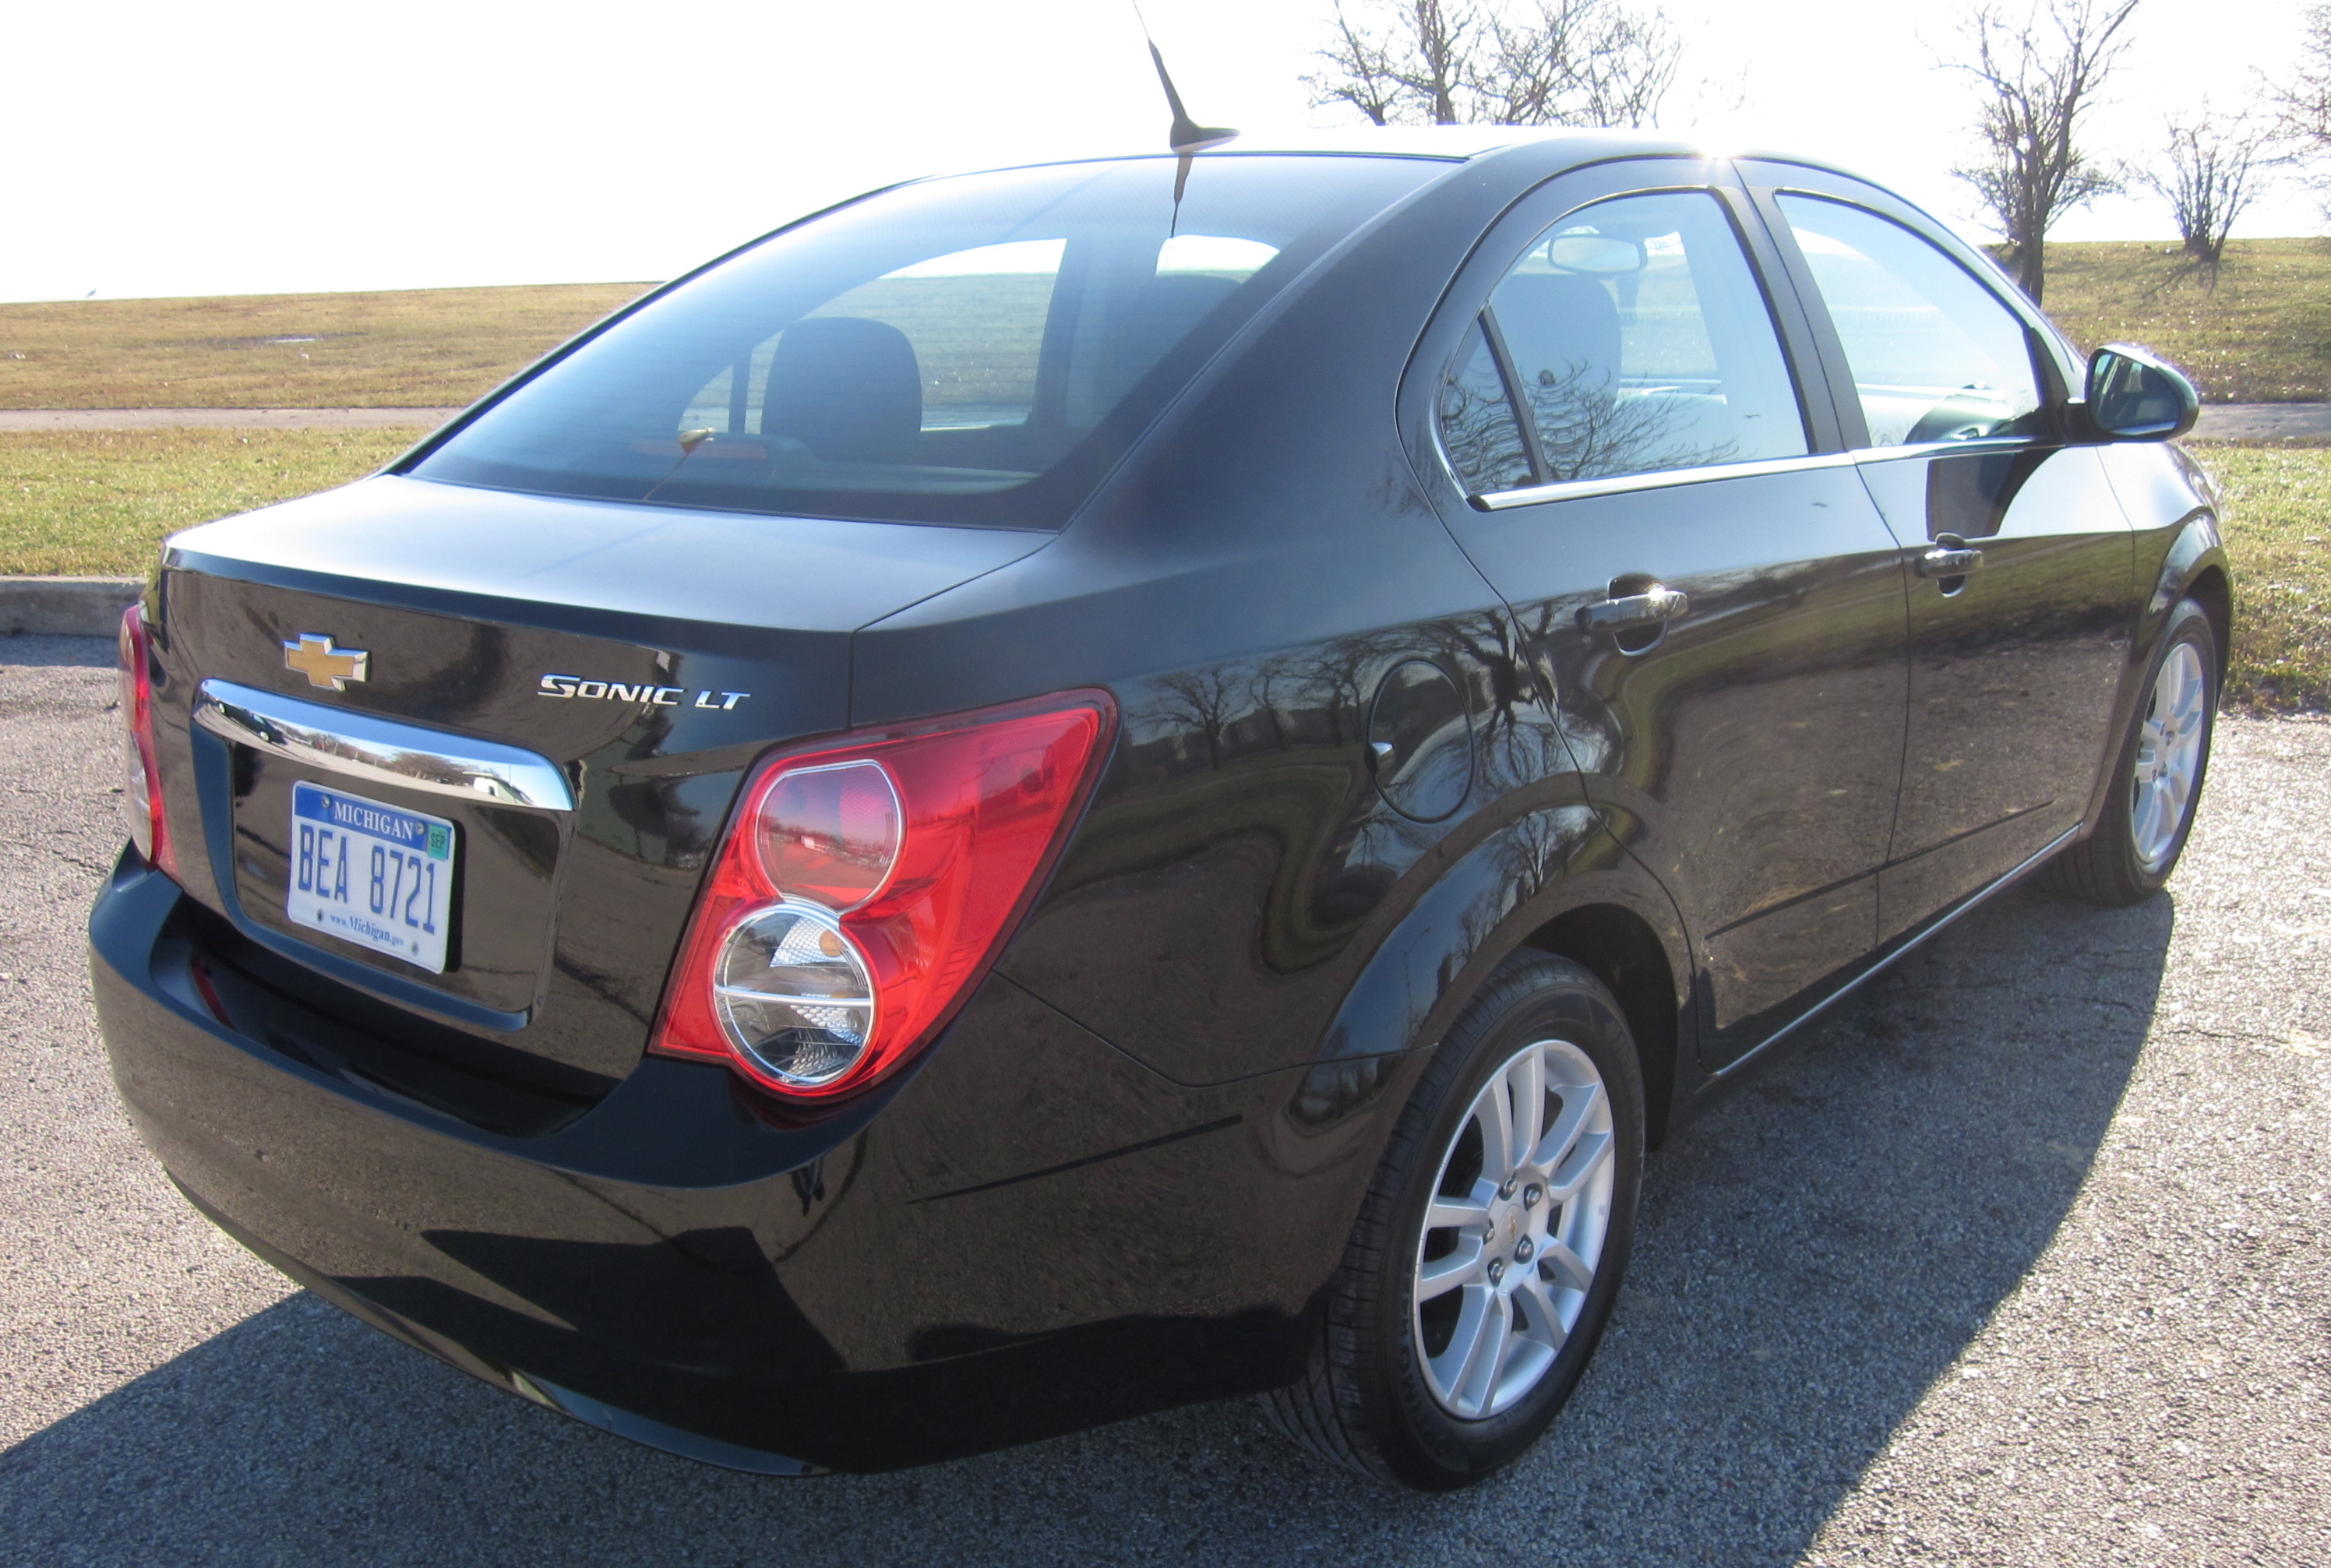
\includegraphics[width=.8\linewidth,height=3cm]{images/images_anomalies/inlier-2}
		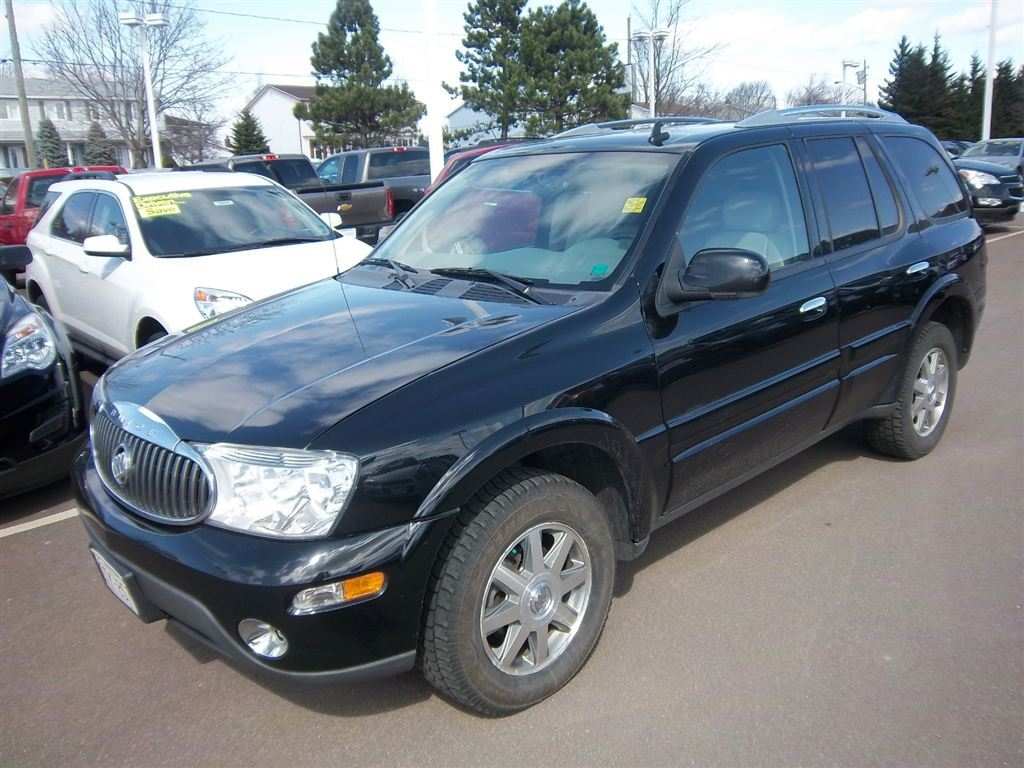
\includegraphics[width=.8\linewidth,height=3cm]{images/images_anomalies/inlier-3}
		\caption{Images "normales"}
		\label{fig:sfig1}
	\end{subfigure}%
	\begin{subfigure}{.33\textwidth}
		\centering
		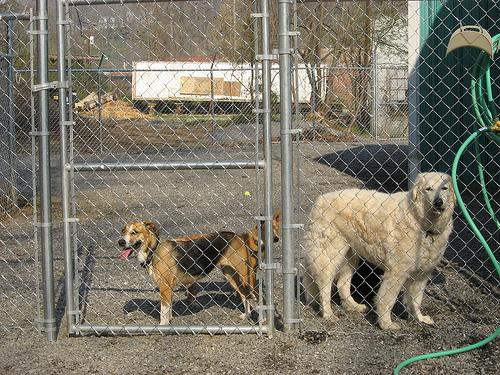
\includegraphics[width=.8\linewidth,height=3cm]{images/images_anomalies/anomalie-1}
		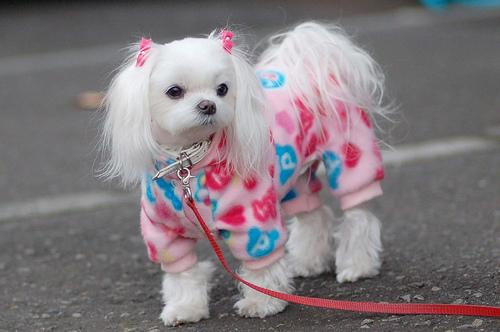
\includegraphics[width=.8\linewidth,height=3cm]{images/images_anomalies/anomalie-2}
		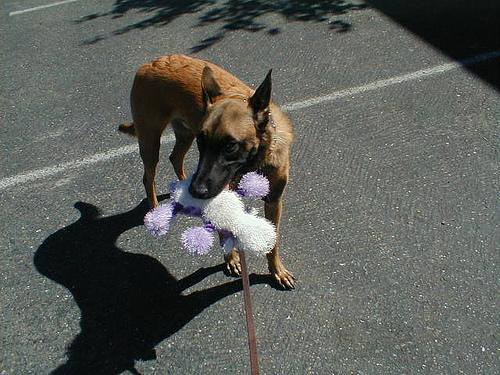
\includegraphics[width=.8\linewidth,height=3cm]{images/images_anomalies/anomalie-3}
		\caption{Images "anormales"}
		\label{fig:sfig2}
	\end{subfigure}
	\begin{subfigure}{.33\textwidth}
		\centering
		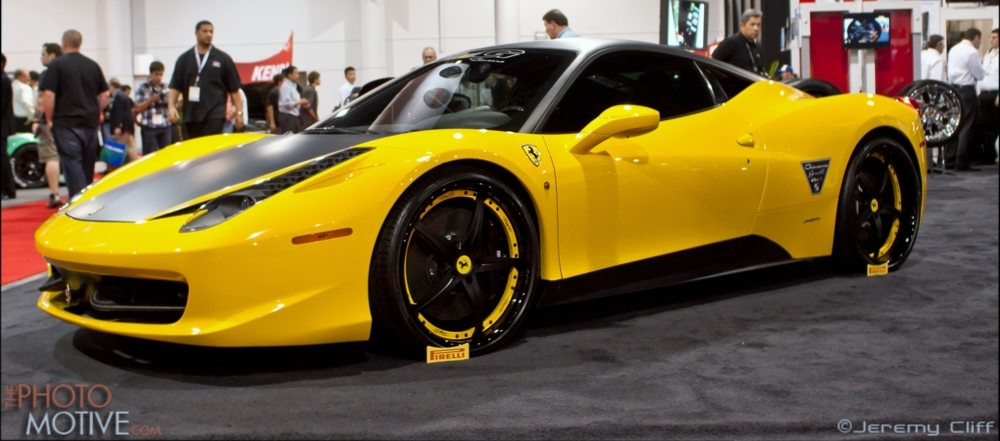
\includegraphics[width=.8\linewidth,height=3cm]{images/images_anomalies/inlier-4}
		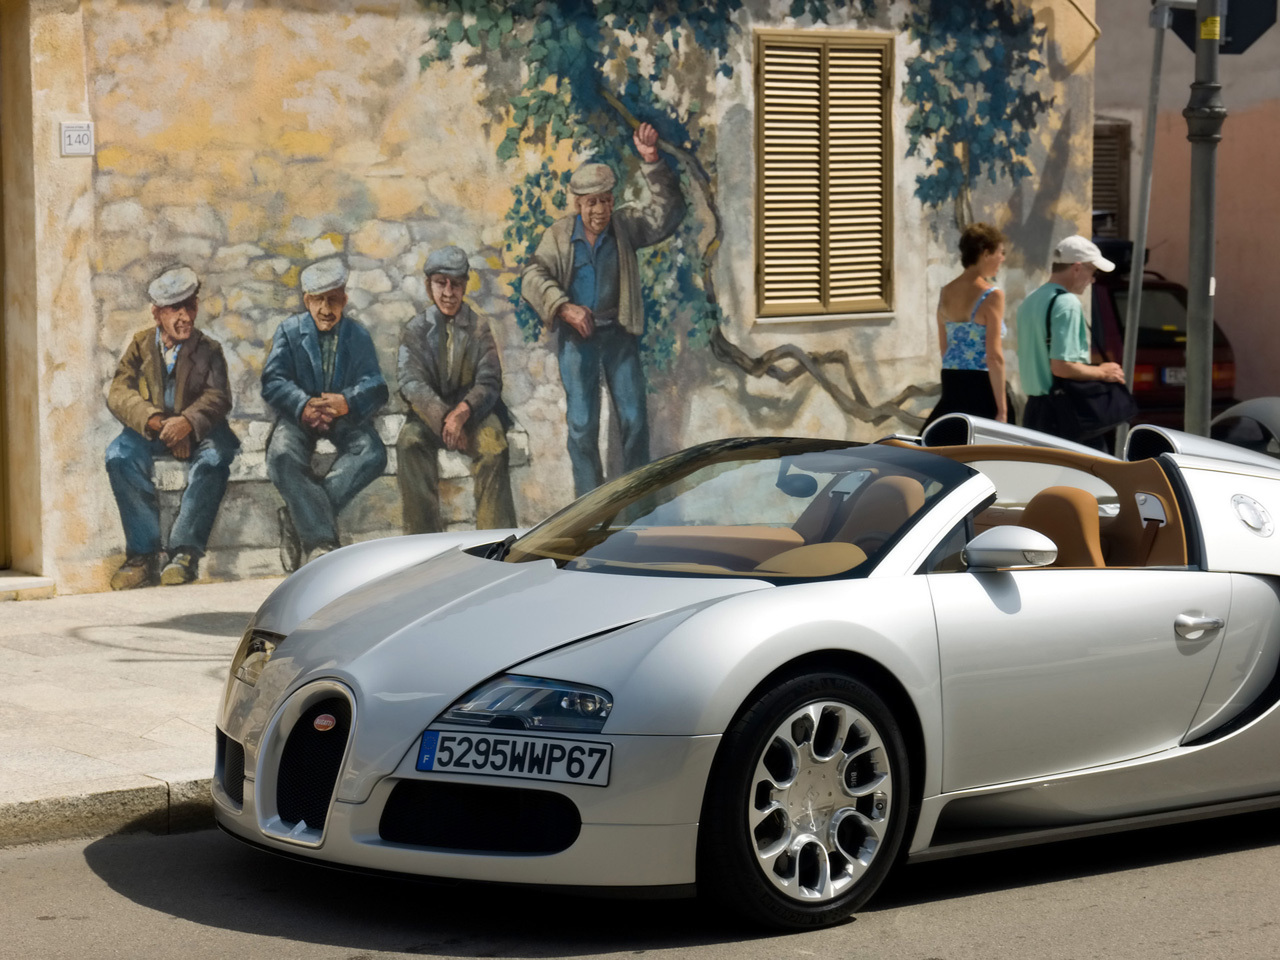
\includegraphics[width=.8\linewidth,height=3cm]{images/images_anomalies/inlier-5}
		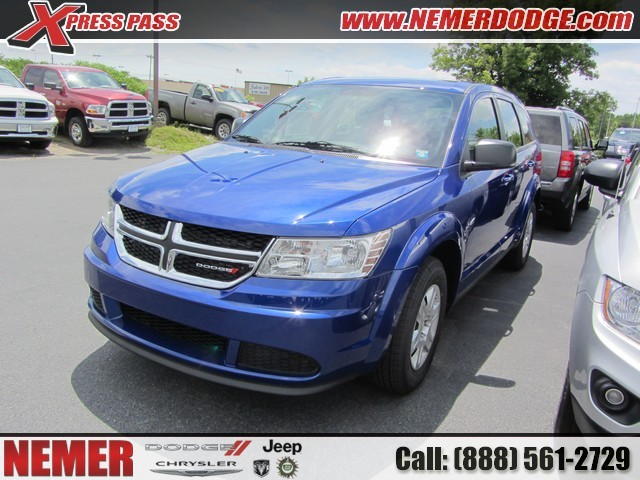
\includegraphics[width=.8\linewidth,height=3cm]{images/images_anomalies/inlier-6}
		\caption{Images "normales"}
		\label{fig:sfig3}
	\end{subfigure}
	\centering
	\caption{Figure illustrant des exemples d'images considérées comme "normales" et d'autres comme "anormales". Dans ce cas, les images dites "normales" sont des images de voitures.}
	\label{fig:exemple_global}
\end{figure}

 La figure \ref{fig:exemple_global} illustre le fait qu'il devient pertinent de trouver une manière d'accorder plus d'importance au contenu global de l'image. Pour ce faire, on utilise un concept qui s'appelle \textit{perceptual loss}. Dans ce type d'optimisation, on calcule la perte en se basant sur une couche spécifique d'un autre réseau de neurones pré-entraîné sur beaucoup plus d'images. En pratique, on utilise généralement des architectures de réseaux connus,  comme \textit{VGG} \citep{DBLP:journals/corr/SimonyanZ14a}  ou \textit{ResNet} \citep{DBLP:journals/corr/HeZRS15}, pré-entraînés sur \textit{ImageNet} \citep{deng2009imagenet}. Cette approche est d'ailleurs utilisée pour transformer le style d'une image, par exemple pour donner le style d'un peintre célèbre à une image quelconque \citep{Johnson2016Perceptual}. La figure \ref{fig:perceptual} illustre le mécanisme exact du calcul de la perte. On peut y voir que l'erreur de reconstruction du réseau n'est plus calculée directement entre la sortie du réseau $\hat{x}$ et l'entrée $x$. En effet, les deux composantes sont plutôt données en entrée à un autre réseau, et l'erreur est calculée en comparant plutôt une représentation précise de ce réseau obtenue par ces deux composantes.

\begin{figure}[h]
	\centering
	\begin{tikzpicture}[shorten >=1pt,draw=black!50, node distance=\layersep, square/.style={regular polygon,regular polygon sides=4}]
	\tikzstyle{neuron}=[circle,fill=black!25,minimum size=30pt,inner sep=0pt]
	\tikzstyle{network}=[square,fill=black!25,minimum size=75pt,inner sep=0pt]
	\tikzstyle{input neuron}=[neuron, fill=green!50];
	\tikzstyle{graph}=[network, fill=white, draw=black];
	\tikzstyle{hidden neuron}=[neuron, fill=blue!50];
	\tikzstyle{annot} = [text width=4em, text centered]
	
	% Draw input (x)
	\node[input neuron] (input) at (0,-5) {$\boldsymbol{x}$};
	
	% Draw the VAE 
	\node[graph] (vae) at (3,-2.5) {$p_{\phi}\{q_{\theta}(\boldsymbol{x})\}$};
	
	% Draw the output (\hat(x)) with x below
	\node[hidden neuron] (x_chap) at (6,-2.5) {$\hat{\boldsymbol{x}}$};
	%\node[input neuron] (input-2) at (6,-5) {$\boldsymbol{x}$};
	
	% Draw the VGG16
	\node[graph] (vgg16_1) at (9,-2.5) {$g(\cdot)$};
	\node[graph] (vgg16_2) at (9,-5) {$g(\cdot)$};
	
	
	% Draw the outputs
	\node[hidden neuron] (input_sortie) at (12,-2.5) {$g(\hat{\boldsymbol{x}})$};
	\node[input neuron] (x_chap_sortie) at (12,-5) {$g(\boldsymbol{x})$};
	
	% Draw arrows
	\path[->, line width=1mm] (input) edge (vae);
	\path[->, line width=1mm] (vae) edge (x_chap);
	\path[->, line width=1mm] (input) edge (vgg16_2);
	\path[->, line width=1mm] (x_chap) edge (vgg16_1);
	\path[->, line width=1mm] (vgg16_1) edge (input_sortie);
	\path[->, line width=1mm] (vgg16_2) edge (x_chap_sortie);
	
	% Annotate the steps
	\node[annot,above of=input, node distance=4.5cm] (h1) {Image d'entrée};
	\node[annot,above of=vae, node distance=2cm] (h2) {VAE};
	\node[annot,above of=vgg16_1, node distance=2cm] (h3) {VGG16*};
	\end{tikzpicture}
	\caption[Figure montrant le mécanisme derrière le concept de \textit{perceptual optimization}]{Figure montrant le mécanisme derrière le concept de \textit{perceptual optimization}. Au lieu de calculer la perte entre $\boldsymbol{x}$ et $\hat{\boldsymbol{x}}$, la perte est calculée entre $g(\boldsymbol{x})$ et $g(\hat{\boldsymbol{x}})$. La fonction $g(\cdot)$ permet d'extraire les valeurs d'une couche spécifique d'un autre réseau pré-entraîné, comme par exemple \textit{VGG16} pré-entraîné sur \textit{ImageNet}.}
	\label{fig:perceptual}
\end{figure}

Étant donné que le réseau correspondant à la fonction $g(\cdot)$ dans la figure \ref{fig:perceptual} est pré-entraîné sur plusieurs images réelles, cela nous permet d'extraire une couche qui contient de l'information à plus bas niveau comme la reconnaissance de lignes, des formes précises, des couleurs, etc. Plus la couche sélectionnée est près de l'entrée du réseau, plus l'information utilisée pour calculer la perte sera simple et brute. À l'inverse, si on sélectionne une couche plus près de la sortie, nous serons en mesure de prendre en compte de l'information plus complexe, par exemple des formes particulières \citep{Johnson2016Perceptual}. L'erreur de reconstruction qui était définie à l'équation \ref{eq:mse_loss} peut maintenant se définir comme suit:

\begin{gather} \label{eq:perceptual_loss}
L(\boldsymbol{x}^{(i)}, p_\phi\{q_\theta(\boldsymbol{x}^{(i)})\}) = \frac{1}{d^2} \sum_{l=1}^{d^2} \Big[g(x^{(i)})_{l} - g(p_\phi\{q_\theta(\boldsymbol{x}^{(i)})\})_{l}\Big]^2.
\end{gather}

L'objectif d'utiliser ce type de perte est d'optimiser la reconstruction du réseau non pas sur les valeurs précises des pixels reconstruites en sortie, mais plutôt sur des représentations contenant de l'information plus structurée. Cela permet entre autres d'orienter l'apprentissage vers la reconstruction du contenu à plus haut-niveau, plutôt que sur la reconstruction parfaite de chaque pixel. Il est important de rappeler que notre objectif est de trouver des anomalies, et non reconstruire parfaitement des images.

Une fois l'autoencodeur variationnel entraîné, c'est-à-dire lorsque les paramètres $\theta$ et $\phi$ sont fixés, il nous est donc possible d'utiliser la partie encodeur du réseau, $q_{\theta}(\cdot) $, pour transformer les images, ou les données en entrée, en une paire de vecteurs $(\boldsymbol{\mu}, \boldsymbol{\sigma})$:

\begin{gather*}  \label{eq:encodeur}
q_{\theta}(\boldsymbol{x}) = (\boldsymbol{\mu}, \boldsymbol{\sigma}), \qquad \boldsymbol{\mu} \in \mathbb{R}^m, \boldsymbol{\sigma} \in \mathbb{R}^m.
\end{gather*}

Certains détails supplémentaires concernant l'entraînement de l'autoencodeur variationnel seront décrits dans la section \ref{DA_VAE}.


\subsection{Définir le cadre décisionnel} \label{cadre_decisionnel}

La prochaine étape de notre approche consiste à définir un cadre décisionnel nous permettant de discriminer les anomalies des observations "normales". Avec ce cadre décisionnel, on cherche à savoir si une observation provenant du jeu de données test, soit $\boldsymbol{X}^{*}$, provient de la population normale $\mathcal{N}$. Pour ce faire, nous allons définir une métrique ou une statistique de distance, obtenue via une fonction $T(\cdot)$, que nous pourrons ensuite comparer à un seuil de décision $s$. La valeur de la statistique de distance et le seuil nous permettront de définir une région $R_{N}=\{x :T(x)<s\}$, pour un $s>0$. Si une observation $\boldsymbol{x^{(i)}}$ se retrouve dans cette région $R_{N}$, nous pourrons supposer que celle-ci est de la population $\mathcal{N}$, donc poser $\hat{\delta}^{*}_{i}=0$. Afin de prendre en compte l'apprentissage fait par l'autoencodeur variationnel, la statistique de distance sera basée sur la représentation latente obtenue par l'encodeur $q_\theta(\cdot)$ pour une observation $\boldsymbol{x^{(i)}}$. Cela nous permet de réécrire la région $R_N$ ainsi:

\begin{gather*}  \label{eq:region}
R_{N}=\{x :T(q_\theta(\boldsymbol{x^{(i)}}))<s\}.
\end{gather*}

Pour obtenir cette région $R_N$, il faut donc procéder en deux étapes. La première consiste à calculer la statistique de distance, donnée par la fonction $T(\cdot)$, sur chacune des instances de notre jeu de données d'entraînement. La deuxième étape consiste à calculer le seuil $s$, ce que nous ferons plus bas à l'aide d'un niveau de filtration $\alpha$ similaire à un niveau de confiance. Ces deux étapes nous permettront de définir notre région de décision nous permettant d'inférer quelles observations du jeu de données test devraient être étiquetées comme des anomalies. Les prochaines sections décrivent plus en détails comment calculer les statistiques de distance et comment définir le seuil à partir de celles-ci.

\subsubsection{Définir une statistique de distance}

 À partir de la section \ref{meth:train-vae}, nous sommes en mesure d'obtenir des représentations latentes, encodées sous forme de vecteurs, pour chaque instance de notre jeu de données $\mathcal{X}$. Nous allons utiliser ces représentations latentes pour générer une statistique de distance selon laquelle nous prévoyons un comportement différent selon qu'une observation est "normale" ou "anormale". La métrique que nous avons choisie pour définir notre statistique de distance est la distance de Kullback-Leibler entre une loi $N(\boldsymbol{\mu}, \boldsymbol{\sigma})$ et une loi $N(0,I)$, où les vecteurs $(\boldsymbol{\mu}, \boldsymbol{\sigma})$ correspondent à la représentation latente obtenue par l'autoencodeur variationnel. Cette statistique de distance, que nous appellerons $T$, est donc définie comme suit pour une observation $i$:
 
 \begin{gather*}  \label{eq:metrique}
 T^{(i)} = D_{KL}\big[N(\boldsymbol{\mu^{(i)}}, \boldsymbol{\sigma^{(i)}}) || N(0, I)\big],
 \end{gather*}
 
 qui permet donc de quantifier la distance entre les vecteurs $(\boldsymbol{\mu^{(i)}}, \boldsymbol{\sigma^{(i)}})$ de la représentation latente d'une observation $i$ et les vecteurs $(\boldsymbol{0_m}, \boldsymbol{1_m})$ correspondant aux paramètres d'une loi $N(0,I)$. Nous pouvons donc calculer cette distance pour chacune des $n$ observations du jeu de données d'entraînement $\mathcal{X}$ pour obtenir l'ensemble de valeurs $T_{\mathcal{X}}=\{T^{(1)}, ..., T^{(n)}\}$. Le raisonnement derrière le choix de cette métrique réside dans le fait que celle-ci est utilisée comme composante dans le critère de perte utilisé lors de l'entraînement de l'autoencodeur. Si l'importance relative de cette composante de perte est différente entre les anomalies et les observations "normales", cette différence devrait se refléter dans les représentations latentes, donc aussi dans la statistique de distance calculée. Le débalancement naturel des anomalies dans un jeu de données nous amène à faire l'hypothèse que les deux composantes de perte ne seront pas optimisées de manière similaire entre les anomalies et les observations "normales".
 
 Maintenant que nous avons fait l'hypothèse que les valeurs des statistiques de distance des anomalies différeront des valeurs des statistiques de distance des observations "normales", il reste à savoir si une valeur élevée est un signe d'anomalie ou l'inverse. Pour savoir comment interpréter la valeur de la statistique, il faut inspecter certaines observations du jeu de données d'entraînement. Nous proposons d'analyser certaines observations ayant des statistiques de distance élevées et certaines observations ayant des statistiques de distance faibles. En analysant les deux extrémités, nous serons en mesure de conclure comment les représentations latentes des observations dites "normales" se comportent par rapport à la loi $N(0,I)$. 
 
 Nos expérimentations révèlent deux scénarios possibles par rapport au comportement des représentations latentes d'observations "normales" par rapport à la $N(0,I)$:

\begin{enumerate} \label{liste_scenarios}
	\item \textbf{Près de la $N(0,I)$:} Les valeurs des statistiques de distance correspondant aux observations "normales" sont faibles dans l'ensemble $T_{\mathcal{X}}$.
	\item \textbf{Éloigné de la $N(0,I)$:} Les valeurs des statistiques de distance correspondant aux observations "normales" sont élevées dans l'ensemble $T_{\mathcal{X}}$.
\end{enumerate}

Les deux scénarios décrits ci-dessus sont illustrés en exemple dans la figure \ref{fig:scenarios}. Dans cette figure, on peut voir le paramètre $\mu$ sur l'axe des $x$ et le paramètre $\sigma^2$ sur l'axe des $y$, ce qui représenterait le cas où les représentations latentes auraient une seule dimension, soit une valeur générée par une loi $N(\mu, \sigma^2)$. On peut y voir la différence par rapport au point central (les deux croix noires) entre les observations connues "normales" (les points rouges) et les observations connues "anormales" (les points bleus).  La marque en forme de "+" correspond au point central des observations "normales" et la marque en forme de "x" correspond au point central des observations "anormales". Cette figure illustre le cas où l'on connait l'étiquette de toutes les observations. Dans un cas réel, nous ne connaitrons pas ces étiquettes et il faudra donc tenter de déterminer lequel de ces deux scénarios semble le plus plausible en analysant certaines observations étant très près et très éloignés du point central $(\boldsymbol{0_m}, \boldsymbol{1_m})$.

\begin{figure} [h]
	\centering
	\begin{subfigure}{6cm}
		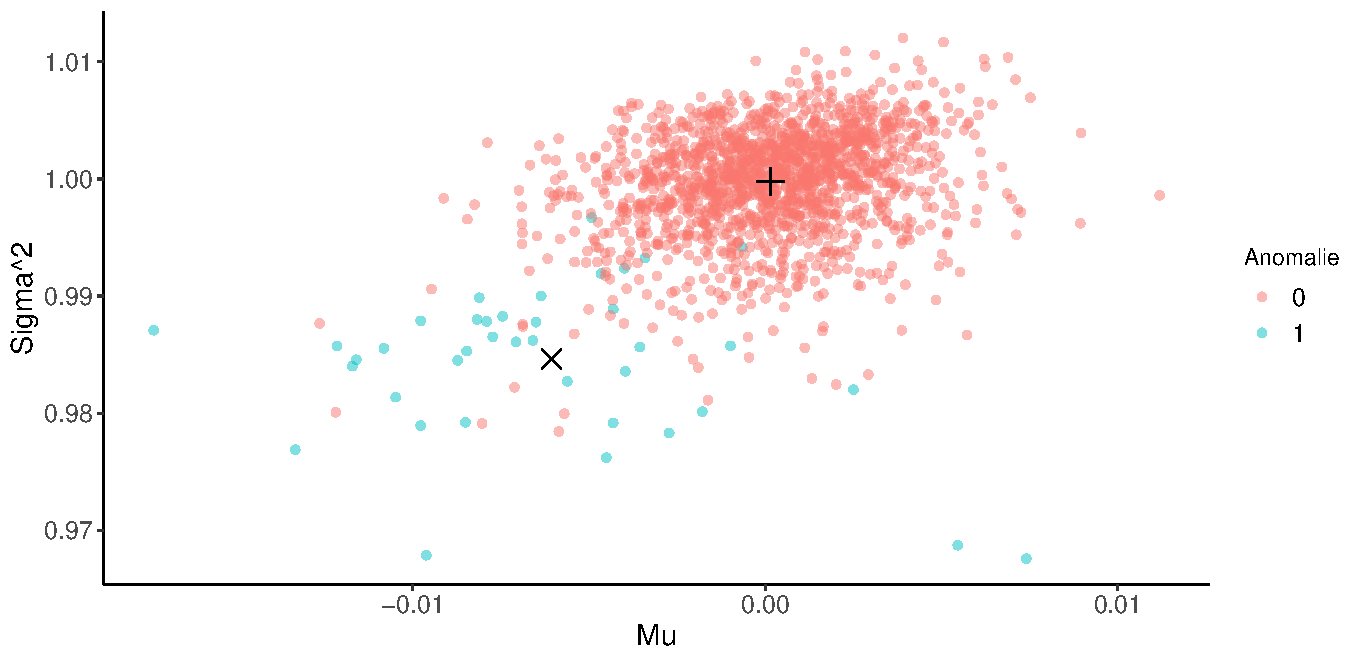
\includegraphics[width=6cm]{images/plot_near.pdf}
		\caption{Scénario 1}
	\end{subfigure}
	\begin{subfigure}{6cm}
		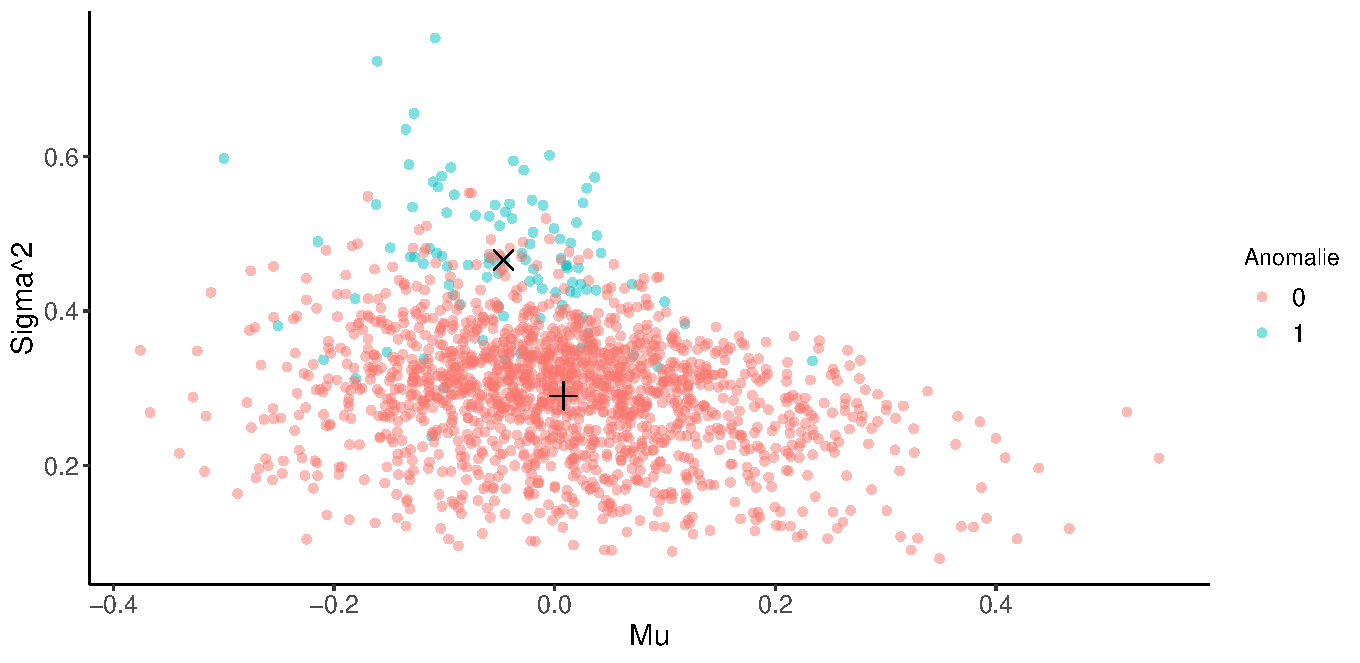
\includegraphics[width=6cm]{images/plot_away.pdf}
		\caption{Scénario 2}
	\end{subfigure}
	\caption{Exemples de situations représentant les deux différents scénarios se rapportant  aux représentation latentes des observations "normales" et "anormales".}
	\label{fig:scenarios}
\end{figure}

Une fois que nous avons défini et analysé les statistiques de distance obtenues sur l'ensemble d'entraînement, nous pouvons passer à la prochaine étape qui consiste à trouver le seuil $s$ nous permettant de définir la région de décision $R_N$.

\subsubsection{Trouver le seuil $s$}

 Pour trouver le seuil $s$, on va utiliser un niveau de filtration $\alpha$ similaire à un niveau de confiance. Ce niveau de filtration $\alpha$ nous permettra de déterminer le seuil $s$. Le seuil déterminé avec un niveau de filtration $\alpha$ sera appelé $s_{(1-\alpha)}$. Par exemple, avec un niveau de filtration $\alpha=0.05$, notre seuil $s_{0.95}$ nous permettra d'identifier les observations ayant des statistiques de distances se retrouvant dans les $95\%$ plus "normales" de l'ensemble d'entraînement $\mathcal{X}$. En faisant varier ce paramètre $\alpha$, nous pourrions identifier plus ou moins d'anomalies. Dans le cas où la proportion d'anomalies $p$ est connue et la même dans  $\mathcal{X}$ et $\mathcal{X}^*$, il est logique de fixer $\alpha=p$.

Pour fixer la valeur du  seuil $s_{(1-\alpha)}$, nous allons extraire une valeur de notre ensemble de statistiques de distance $T_{\mathcal{X}}$. Nous pourrons ensuite comparer cette valeur $s_{(1-\alpha)}$ à la valeur d'une statistique de distance  correspondant à une nouvelle observation pour conclure si cette nouvelle observation fait partie de la région $R_N$, que nous dénoterons $R_{N}^{\alpha}$ pour rendre explicite la dépendance au niveau de filtration $\alpha$. Le scénario identifié à la section précédente nous est nécessaire pour trouver la valeur du seuil $s_{(1-\alpha)}$. Dans le scénario où les observations "normales" sont près de la $N(0,I)$, soit le scénario 1, nous allons préalablement ordonner les valeurs de $T_{\mathcal{X}}$ en ordre croissant. Dans le scénario inverse où les observations "normales" sont éloignées de la $N(0,I)$, soit le scénario 2, nous allons plutôt ordonner les valeurs de $T_{\mathcal{X}}$ en ordre décroissant. Nous définissons $T^{'}_{\mathcal{X}}$, l'ensemble $T_{\mathcal{X}}$ ordonné selon le scénario en question. Le seuil $s_{(1-\alpha)}$ correspond donc à la valeur associée au rang $\lfloor(1 - \alpha) \times n\rfloor$ de l'ensemble $T^{'}_{\mathcal{X}}$:

\begin{gather*} \label{eq:seuil}
s_{(1 - \alpha)} = T^{'}_{\mathcal{X} \{(1 - \alpha) \times n\}},
\end{gather*}

où $T^{'}_{\mathcal{X} \{(1 - \alpha) \times n\}}$ est la valeur correspondant au rang $\lfloor(1 - \alpha) \times n\rfloor$ de l'ensemble $T^{'}_{\mathcal{X}}$. Ce seuil nous permet de définir la région $R_{N}^{\alpha}$, qui représente la région où une observation est considérée comme "$(1-\alpha)-$normale". Si on définit $t$ comme étant la valeur d'une statistique de distance calculée comme $t = T(q_\theta(\boldsymbol{x}))$, la région $R_{N}^{\alpha}$ est donnée par:

\begin{gather*} \label{eq:region}
	R_{N}^{\alpha} = 
	\begin{cases} 
		\big\{t \in \mathbb{R}: t < s_{(1 - \alpha)} \big\} & \text{si les observations "normales" sont près de $N(0, I)$}, \\
		\big\{t \in \mathbb{R}: t > s_{(1 - \alpha)} \big\} & \text{si les observations "normales" sont éloignées de $N(0, I)$}.
	\end{cases}
\end{gather*}

Pour étiqueter les observations de notre jeu de données test, nous allons calculer les statistiques de distance $T$ des $k$ observations de ce jeu de données $\mathcal{X^*}$. Si la valeur de la statistique de distance $T^{(j)}$ correspondant à l'observation $\boldsymbol{x^{*(j)}}$ fait partie de la région $R_{N}^{\alpha}$, on peut donc conclure que l'observation fait partie de "ensemble $(1-\alpha)$-normal". Si la statistique de distance $T^{(j)}$ ne fait pas partie de la région $R_{N}^{\alpha}$, on l'étiquettera comme une "$\alpha$-anomalie".

La région $R_{N}^{\alpha}$ nous permet de définir si une observation est une $\alpha$-anomalie ou non. De manière similaire, on peut également utiliser l'ensemble $T_{\mathcal{X}}$ pour établir un score d'anomalie pour une observation donnée. Ce score d'anomalie est défini entre $[0,1]$, où une anomalie évidente devrait avoir un score se rapprochant de 1. Pour établir ce score, il faut calculer la statistique de distance $T^{(j)}$ correspondant à l'observation $\boldsymbol{x^{*(j)}}$, ensuite calculer le rang de cette statistique de distance parmi l'ensemble $T^{'}_{\mathcal{X}}$ et finalement diviser ce rang par le nombre d'observations $n$ dans l'ensemble $T^{'}_{\mathcal{X}}$. Ce score d'anomalie, dénoté $\gamma$, pour une observation $\boldsymbol{x^{*(j)}}$ est donné par

\begin{gather} \label{eq:score_anomalie}
	\gamma(\boldsymbol{x^{*(j)}}) = \frac{rang_{T^{'}_{\mathcal{X}}}(T^{(j)})}{n},
\end{gather}

où $rang_{T^{'}_{\mathcal{X}}}(T^{(j)})$ correspond au rang de la statistique de distance $T^{(j)}$ dans l'ensemble ordonné $T^{'}_{\mathcal{X}}$. Une valeur élevée du score défini à l'équation \ref{eq:score_anomalie}, ou près de 1, signifie que l'observation $\boldsymbol{x^{*(j)}}$ est considérée comme une anomalie selon l'algorithme.

L'algorithme \ref{alg:metho} résume les différentes étapes de notre approche.

\begin{center}
	\begin{algorithm}[H] \label{alg:metho}
		\SetAlgoLined
		\KwIn{Ensemble de données d'entraînement $\boldsymbol{x^{(i)}}, i=1,...,n$ \\ Ensemble de données de test $\boldsymbol{x^{*(j)}}, j=1, ..., k$
		\\ Niveau de filtration $\alpha$}
		\KwOut{Indicateurs d'$\alpha$-anomalies $\hat{\delta}^{(j)}_{\alpha}, j=1,...,k$}
		$\theta$, $\phi$ $\leftarrow$ paramètres de l'encodeur ($q_{\theta}(\cdot)$) et du  décodeur ($p_{\phi}(\cdot)$) du VAE entraîné\;
		\For{i=1 to n}{
			$ (\boldsymbol{\mu^{(i)}}, \boldsymbol{\sigma^{(i)}}) = q_{\theta}(\boldsymbol{x^{(i)}})$ \\
			$T_{\mathcal{X}}^{(i)}=D_{KL}\big[N(\boldsymbol{\mu^{(i)}}, \boldsymbol{\sigma^{(i)}}) || N(0, I)\big]$
		}
		Ordonner $T_{\mathcal{X}}$ selon le scénario identifié pour obtenir $T^{'}_{\mathcal{X}}$ \;
		\For{j=1 to k}{
			$(\boldsymbol{\mu^{(j)}}, \boldsymbol{\sigma^{(j)}}) = q_{\theta}(\boldsymbol{x^{*(j)}})$ \\
			$T_{\mathcal{X^*}}^{(j)}=D_{KL}\big[N(\boldsymbol{\mu^{(j)}}, \boldsymbol{\sigma^{(j)}}) || N(0, I)\big]$ \\
			$\gamma(\boldsymbol{x^{*(j)}}) = rang_{T^{'}_{\mathcal{X}}}(T_{\mathcal{X^*}}^{(j)})/n$ \\
			\eIf{$\gamma(\boldsymbol{x^{*(j)}}) >= (1 - \alpha)$}{
				$\hat{\delta}^{(j)}_{\alpha}$ = $vrai$
			}
			{
				$\hat{\delta}^{(j)}_{\alpha}$ = $faux$
			}
		}
		\KwRet{$\boldsymbol{\hat{\delta}}_{\alpha}$ \text{et} $\gamma(\boldsymbol{x^{*(j)}}, j=1, ..., k)$}
		\caption{Algorithme de détection d'anomalies basé sur les représentations latentes d'un autoencodeur variationnel}
	\end{algorithm}
\end{center}

Cette section conclut la description de notre approche de détection d'anomalies. Dans la prochaine section, nous allons présenter différentes expérimentations mettant en application cette approche.
